\documentclass[tikz,border=12pt]{standalone}
\usepackage{fontspec}
\setmainfont{Segoe UI}
\usepackage{amsmath,amssymb}
\usepackage{tikz}

\usetikzlibrary{calc,arrows.meta}

\begin{document}
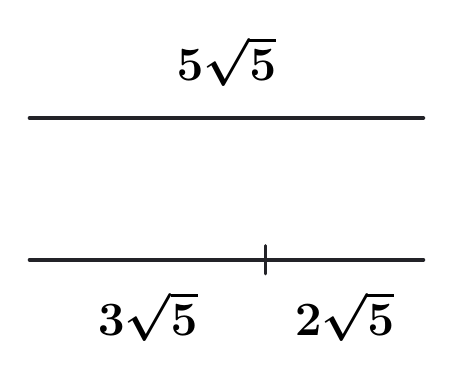
\begin{tikzpicture}[x=1.0000cm,y=1cm,line cap=round,line join=round]
\definecolor{linec0}{RGB}{35,35,40}
\definecolor{linec1}{RGB}{35,35,40}
\definecolor{linec2}{RGB}{35,35,40}
\definecolor{linec3}{RGB}{35,35,40}
\definecolor{linec4}{RGB}{35,35,40}
\definecolor{linec5}{RGB}{35,35,40}
\definecolor{edgecol}{RGB}{35,35,40}
\definecolor{hicol}{RGB}{35,35,40}
\definecolor{angcol}{RGB}{35,35,40}
\coordinate (A) at (0.0000,0.0000);
\coordinate (B) at (3.0000,0.0000);
\coordinate (C) at (5.0000,0.0000);
\coordinate (P) at (3.0000,-0.1800);
\coordinate (Q) at (3.0000,0.1800);
\coordinate (D) at (0.0000,1.8000);
\coordinate (E) at (5.0000,1.8000);
\draw[line width=1.4pt,color={rgb,255:red,35;green,35;blue,40}] (A) -- (B);
\draw[line width=1.4pt,color={rgb,255:red,35;green,35;blue,40}] (B) -- (C);
\draw[edgecol,line width=1.1pt] (P) -- (Q);
\draw[line width=1.4pt,color={rgb,255:red,35;green,35;blue,40}] (D) -- (E);
\node[fill=white,inner sep=3pt,font=\LARGE,text=black] at (1.500,-0.720) {{\boldmath $3\sqrt{5}$}};
\node[fill=white,inner sep=3pt,font=\LARGE,text=black] at (4.000,-0.720) {{\boldmath $2\sqrt{5}$}};
\node[fill=white,inner sep=3pt,font=\LARGE,text=black] at (2.500,2.520) {{\boldmath $5\sqrt{5}$}};
\end{tikzpicture}
\end{document}
